%%% LaTeX Template
%%% This template can be used for both articles and reports.
%%%
%%% Copyright: http://www.howtotex.com/
%%% Date: February 2011

%%% Preamble
\documentclass[paper=a4, fontsize=11pt]{scrartcl}	% Article class of KOMA-script with 11pt font and a4 format
\usepackage[margin=0.7in]{geometry}
\usepackage[english]{babel}															% English language/hyphenation
\usepackage[protrusion=true,expansion=true]{microtype}				% Better typography
\usepackage{amsmath,amsfonts,amsthm}										% Math packages
\usepackage[pdftex]{graphicx}														% Enable pdflatex
%\usepackage{color,transparent}													% If you use color and/or transparency
\usepackage[hang, small,labelfont=bf,up,textfont=it,up]{caption}	% Custom captions under/above floats
\usepackage{epstopdf}																	% Converts .eps to .pdf
\usepackage{subfig}																		% Subfigures
\usepackage{booktabs}																	% Nicer tables

%%% Advanced verbatim environment
\usepackage{verbatim}
\usepackage{fancyvrb}
\DefineShortVerb{\|}								% delimiter to display inline verbatim text


%%% Custom sectioning (sectsty package)
\usepackage{sectsty}								% Custom sectioning (see below)
\allsectionsfont{%									% Change font of al section commands
	\usefont{OT1}{bch}{b}{n}%					% bch-b-n: CharterBT-Bold font
%	\hspace{15pt}%									% Uncomment for indentation
	}

\sectionfont{%										% Change font of \section command
	\usefont{OT1}{bch}{b}{n}%					% bch-b-n: CharterBT-Bold font
	\sectionrule{0pt}{0pt}{-5pt}{0.8pt}%	% Horizontal rule below section
	}


%%% Custom headers/footers (fancyhdr package)
\usepackage{fancyhdr}
\pagestyle{fancyplain}
\fancyhead{}														% No page header
\fancyfoot[C]{\thepage}										% Pagenumbering at center of footer
\renewcommand{\headrulewidth}{0pt}				% Remove header underlines
\renewcommand{\footrulewidth}{0pt}				% Remove footer underlines
\setlength{\headheight}{13.6pt}

%%% Equation and float numbering
\numberwithin{equation}{section}															% Equationnumbering: section.eq#
\numberwithin{figure}{section}																% Figurenumbering: section.fig#
\numberwithin{table}{section}

\usepackage[parfill]{parskip}
\usepackage{float}
\usepackage{graphicx}
\usepackage{hyperref}
\usepackage[numbers]{natbib}															% Tablenumbering: section.tab#
\usepackage{minted}
\usepackage[toc,page]{appendix}



%%% Title	
\title{ \vspace{-1in} 	\usefont{OT1}{bch}{b}{n}
		\huge \strut VESUVIO Data Reduction and Analysis in Mantid \strut \\
}
\author{ 									\usefont{OT1}{bch}{m}{n}
        Samuel Jackson\\		\usefont{OT1}{bch}{m}{n}
        ISIS Facility\\	\usefont{OT1}{bch}{m}{n}
        Rutherford Appleton Laboratory\\
        \texttt{samuel.jackson@stfc.ac.uk}
}
\date{\today}

%%% Begin document
\begin{document}
\maketitle
\clearpage
\tableofcontents
\clearpage

\section{Abstract}
VESUVIO is a neutron spectrometer at the ISIS pulsed neutron source operating at high energies in the 1 eV range and uses the experimental technique known as neutron Compton scattering to measure the momentum distributions of condensed matter systems \citep{mayers2012vesuvio}. Mantid \citep{mantid} is a data analysis application for neutron and muon scattering data used by multiple facilities across the world. Recently, extensive work has been carried out to integrate the bespoke data reduction and analysis routines written for VESUVIO with the Mantid framework. While the programs described in this document are designed to replicate the functionality of the Fortran and Genie routines already in use, most of them have been written from scratch and are not based on the original code base. This document outlines the current progress of development regarding what has already been implemented and what is remains to be finished.

\clearpage
\section{Introduction}
\label{sec:introduction}
\subsection{VESUVIO Overview}
\label{subsec:VESUVIO-overview}
VESUVIO is a deep inelastic neutron scattering spectrometer situated on the S2 beamline at ISIS with an operational energy range of 5-150 eV. The instrument utilises a indirect geometry design and consists of 64 Yttrium Aluminium Perovskite $\gamma$-ray forward scattering detectors in 8 separate banks and 132 $^6$Li doped glass scintillator back scattering detectors split into 3 banks. The scattered neutron beam impinges onto the analyzer foil which provides the energy analysis by means of resonance absorption at a given resonance energy. For this purpose usually gold foils are employed which have a large energy resonance at 4.9 eV $\pm$ 0.15 eV. With this experimental arrangement, data collection necessarily involves foil cycling in both forward and backscattering geometries in order to obtain TOF data with and without energy selection, followed by a subtraction of these two data sets to obtain NCS spectra. 

In this context, it is worth emphasizing that the “foil-out” data set in every VESUVIO experiment is tantamount to a simultaneous ND measurement of the sample under investigation. On VESUVIO, two different final-energy-selection schemes are currently used, hereafter referred to as resonance-detector (RD) and resonance-filter (RF) configurations. The RD configuration employs the foil to define the energy of the scattered neutrons via resonant neutron absorption, and a $\gamma$-ray detector to probe the prompt cascade following the subsequent (n,$\gamma$) reaction \cite{schooneveld2006foil}. At present, VESUVIO uses RD (RF) in forward (backscattering) geometries, respectively.

\begin{figure}[H]
\centering
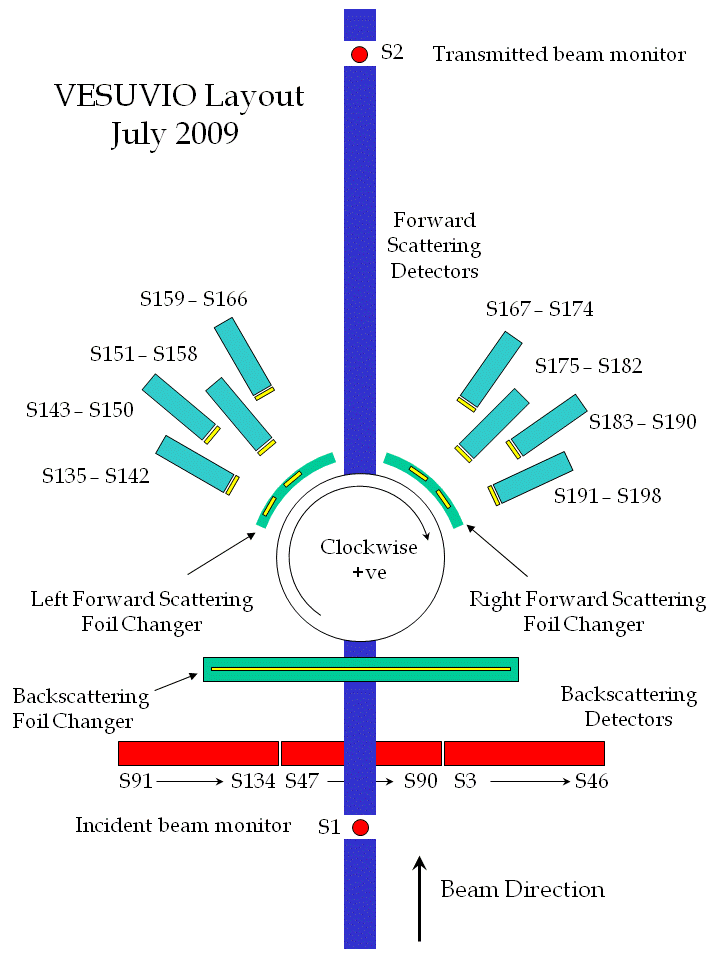
\includegraphics[width=0.5\textwidth]{img/vesuvio-diagram.png}
\caption{Schematic diagram of the VESUVIO instrument. Positions of the gold foils used for each of the differencing methods are shown in yellow.}
\label{fig:VESUVIO-diagram}
\end{figure}

For the RF configuration, the VESUVIO backscattering bank is equipped with Li-doped glass detectors only sensitive to neutrons \cite{seeger1985double} and the TOF spectra are obtained by taking the difference between “foil-in” and “foil-out” data, referred to as single difference (SD). To improve final-energy resolution, double-difference (DD) techniques have been implemented with three measurements, namely with no filter, a filter of thickness d1 and neutron absorption A1(E1) and a filter of the same material of thickness d2 and absorption A2(E1). The energy resolution function is well approximated by a Voigt line shape where the Lorentzian contribution is largely removed by the DD technique.

VESUVIO is primarily designed to measure the atomic momentum distribution of atoms in condensed matter systems. Data analysis on VESUVIO relies on the accuracy of two approximations, namely the incoherent (INCA) and impulse approximation (IA). INCA implies that for incident neutron wavelengths much less than the d-spacing of the sample, atoms will scatter incoherently and the measured intensity is
therefore the total sum of intensities for individual atoms in the sample \cite{fernandezalonso2013neutron}. IA effectively treats the scattering as single atom `billiard ball' scattering, with conservation of momentum and kinetic energy of and a neutron a single target atom, allowing the momentum distribution of a mass to be measured using the theory developed in Ref. \cite{mayers2012vesuvio}. 

NCS data contains a number of spectra each consisting of a series of peaks. Each of these peaks corresponds to a single atomic mass in the sample being studied. The positions of the peaks in the spectrum are determined by the mass of the sample. The amplitude of each of the peaks is determined by an atom's mass and scattering cross section. Finally, the width of the peaks is determined by the momentum distribution of the mass. The goal of data analysis of VESUVIO data is to determine the shape and intensity of the peaks, thereby determining the momentum distributions of the atoms in the sample. \cite{mayers2010user}.

\subsection{Introduction to the NCS data analysis module}
\label{subsec:intro-data-analysis}
The Mantid development team in combination with VESUVIO instrument scientists have created a data analysis package to help aid with the analysis of VESUVIO data. This is still a work in progress and under heavy development. Currently it is in the form of a separate python module called ncs.py (NCS: Neutron Compton Scattering) which provides a collection of helper functions and classes for data analysis which builds upon the existing Mantid framework. This module is publicly available in the Mantid Github scripts repository in the \textit{development \textgreater  inelastic} folder \cite{mantidgithubncs}. The simplest way of including the ncs python module in Mantid is to place the files \textit{ncs.py} and \textit{ncs\_plotting.py} in the \textit{ \textless Mantid Install \textgreater }/\textit{scripts} folder. This will allow the ncs module to be imported directly into the Mantid script window.

\section{Viewing Data in Time-of-Flight}
\label{sec:viewtof}
The original data analysis package \cite{mayers2010user} used two separate commands to process the raw time-of-flight data, one for the frontscattering detectors and one for the backscattering. In the Mantid implementation this has been replaced with a single algorithm called LoadVesuvio which performs all of the processing for raw files from the instrument. This includes options for handling each of the different foil positions and difference techniques available with VESUVIO \citep{schooneveld2006foil, mayers2004vesuvio} and handles summing multiple runs. It also contains a flag for summing each spectrum in the desired range into a single spectrum. The results of this loading operation are output as a single workspace in Mantid with units in time-of-flight which can be plotted using both Mantid's in built visualisation tools and custom plotting commands described in section \ref{sec:visualisation}. Like all inelastic instruments at ISIS, VESUVIO uses time-of-flight measurements to determine the momentum and energy transfer to the neutron in each scattering event. The neutron counting chain assigns a time of flight to the arrival of each neutron at the detector.

\begin{equation}
\label{eq:time-of-flight}
t = \frac{L_0}{v_0} + \frac{L_1}{v_1} + t_0
\end{equation}

$L0$ is the path length from source to sample, $L1$ that from sample to detector, $v0$ is the velocity of the incident neutron and $v1$ that of the scattered neutron. $t0$ is an offset from the true value of due to delays in the electronic counting chain. On VESUVIO the values of $L0$, $L1$, $v1$, $t0$ and the scattering angle can be characterised by a mean value, with an associated distribution about the mean. Given these mean values and the value of $t$ assigned to the neutron, the incident velocity $v0$ of each neutron detected and hence the
momentum and energy transfer in the scattering process can be determined from eq. \ref{eq:time-of-flight} above. The distributions of these parameters about their mean values determine the resolution function of the instrument. The main task instrument calibration procedure is to determine these distributions and store them in the instrument parameter (IP) file.

\begin{figure}[H]
\centering
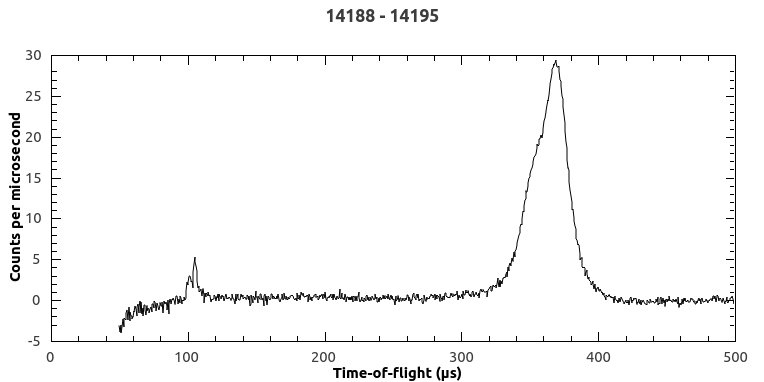
\includegraphics[width=0.6\textwidth]{img/tof-spectrum.png}
\caption{Plot of time-of-flight data from the sum runs 14188-14195 and the sum of detectors 40-134.}
\label{fig:tof-spectrum}
\end{figure}

Optionally, an instrument parameter file can be supplied to the loading routine. This file contains a set of calibrated instrument parameters for each of the detectors and can correct each of the default parameters used and attach the $t0$ parameter to the instrument attached to the workspace. This parameter file is usually generated by the instrument scientist using a set of reference runs using the calibration program outlined in section \ref{sec:calibration} and does not need to be regenerated for every analysis session. 

Once VESUVIO data has been loaded into a Mantid workspace it can be used with the various tools in the ncs data analysis module. Typically the first step after loading the raw data in time-of-flight is to crop the workspace to a sensible range for data analysis. This can be done by using the Mantid CropWorkspace algorithm. The typical time-of-flight range used is 50.0 - 562.0 $\mu s$.

\begin{listing}[H]
\begin{minted}[frame=lines,linenos=true,fontsize=\footnotesize]{python}
import ncs
runs = "14188-14195"
spectra = "134"
diff_type="SingleDifference" # Allowed values=Single,Double,Thick
ip_file = "IP0004_10.par"

raw_ws = LoadVesuvio(Filename=runs, SpectrumList=spectra,
		     Mode=diff_type,InstrumentParFile=ip_file)
raw_ws = CropWorkspace(raw_ws,XMin=50.0,XMax=562.0)
\end{minted}
\caption{Example script showing how to load and crop VESUVIO data using the Mantid python API.}
\label{lst:loading-data}
\end{listing}

The ncs.py module also provides a preprocessing function for further preparing the data for analysis. This method provides options for masking data points in the raw workspace given an error threshold as well as an option to smooth the workspace using the SmoothData algorithm. This requires a \textit{FitOptions} object to be supplied (see section \ref{sec:fitting}).

\section{Multiple Scattering and Gamma Background Corrections}
\label{sec:corrections}
The time-of-flight data loaded using the methods described in section \ref{sec:viewtof} need to be corrected to account for the effects of multiple scattering \citep{mayers2002multiple} and gamma background \citep{mayers2011calculation}. Currently, the multiple scattering corrections for VESUVIO in Mantid are under development and will be available in future releases. When the secondary foil absorbs neutrons it also emits $\gamma$-rays, which can be registered by the YAP detectors. The residual background is non-zero because the intensity of these is different in the two positions occupied by the secondary foil. With the current arrangement of foils and detectors on VESUVIO the residual background is at the ~5\% level compared to the signal.

Corrections for the gamma background are implemented using the Mantid algorithm framework as an algorithm called \textit{CalculateGammaBackground}. This takes a single workspace in time-of-flight, and a fit function describing the mass spectrum of the input data and a list of workspace indices to include as part of the correction. The fit function for the mass spectrum is typically one which has been created as part of the fit routines described in section \ref{sec:fitting}. This algorithm results in two workspaces: one that contains the calculated background and a copy of the input time-of-flight workspace with the background subtracted. This function loosely corresponds to the \textit{bcorr} command in the old data analysis package.

\begin{figure}[H]
\centering
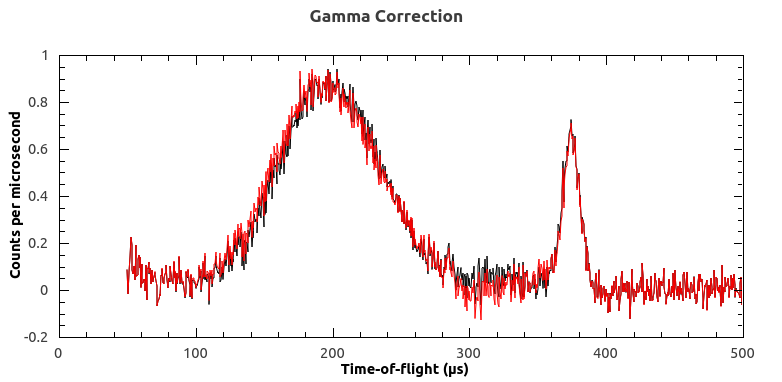
\includegraphics[width=0.6\textwidth]{img/corrections-gamma.png}
\caption{Plot of a Zirconium Hydride (ZrH$_2$) sample. Black is the uncorrected sample, red shows the same sample after gamma correction.}
\label{fig:corrections-gamma}
\end{figure}

There are helper functions for this implemented in ncs.py. The gamma background can be computed from a workspace simply by using the \textit{gamma\_correct} function and passing the raw workspace to correct, the required fitting options, and the parameter workspace produced from a fit (see section \ref{sec:fitting}). Listing \ref{lst:gamma-correction} shows the code to perform a gamma correction on a workspace that has already been fitted.

\begin{listing}[H]
\begin{minted}[frame=lines,linenos=true,fontsize=\footnotesize]{python}
ncs.preprocess(raw_ws, fit_options)
reduced_chi_square, params_ws = ncs.run_fit(raw_ws, fit_options)
ncs.display_fit_output(reduced_chi_square, params_ws, fit_options)

background, corrected = ncs.gamma_correct(raw_ws, fit_options, params_ws)
\end{minted}
\caption{Example script for performing a gamma correction to the ZrH$_2$ sample using ncs.py.}
\label{lst:gamma-correction}
\end{listing}

\section{Fitting}
\label{sec:fitting}
The majority of the work to integrate VESUVIO into Mantid has been concerned with the development of the fitting procedures required to measure the neutron Compton profile following the theory described in Ref. \citep{mayers2012vesuvio}. Development in this area has focussed on two major additions to the Mantid framework. First was the creation a new suite of fit functions which could accurately describe the results of a neutron Compton scattering experiment. The second was the creation of a collection of supporting data analysis functions which allow the user to easily set up a fit given the appropriate parameters for the sample and are available in the ncs.py module. These will eventually be folded into a GUI for VESUVIO (see section \ref{sec:GUI}).

There are two major fit functions used in the analysis of VESUVIO data. The \textit{GaussianComptonProfile} defines a function for fitting the simpler Gaussian approximation to mass peaks. The \textit{GramChalierComptonProfile} is for the more complex fitting case where the atoms in the sample are affected by anisotropy and anharmonicity. The theory behind both of these functions are described in detail in Refs. \cite{mayers2012vesuvio, andreani2005measurement}. Both functions are implemented as standard Mantid fit functions and are therefore directly accessible through the fit wizard.

The fitting routines provided as part of ncs.py are radically different from the originals described in Ref. \cite{mayers2010user}. Currently, in order to run a fit a \textit{FitOptions} object must be created from ncs.py and set up with the appropriate options for the sample being fitted. This includes a set of parameters for each mass describing its atomic weight, the function it should be fitted with and any additional options specific to the model used. Listing \ref{lst:fit-setup} shows an example of how to set up the parameters of a fit using the ncs.py \textit{FitOptions} class. Table \ref{table:fit-parameters} lists all of the current fitting options available in the \textit{FitOptions} class, while table \ref{table:mass-parameters} describes each of the options for defining the masses to be fitted.

\subsection{Fitting the data to obtain sample compositions and kinetic energies}
\label{subsec:fitting-composition-kinetic}

The simplest mode of analysis is to assume that each of the peaks in momentum space is of Gaussian shape \cite{mayers2004vesuvio}. Using the amplitudes and widths obtained for the fit the composition of the sample and the atomic kinetic energies may be determined. Listing \ref{lst:fit-setup} shows a basic example of how to use the \textit{FitOptions} class to set up fit for the aluminium and zirconium masses in the sample.

Fitting the data shown in listing \ref{lst:loading-data} with the parameters defined in listing \ref{lst:fit-setup} produces three workspaces. One containing the fit of the composite function and individual mass profiles to the raw data, a table workspace of parameters for the fit, and a table workspace for the normalised covariance matrix of the fit. These workspaces are in fact just the standard output from the Mantid Fit algorithm. A plot of the fit using the Gaussian approximation function to two mass peaks for aluminium and zirconium is shown in \ref{fig:gaussian-example-fit}. Comparing this to the original example in Ref. \cite{mayers2010user} shows a good correlation between implementations.

The fitted amplitudes and widths of the sample can be examined by looking at the parameters table produced by the fit. In the original VMS data analysis package a routine called \textit{ke} was used to calculate the kinetic energy in meV and K and the fundamental frequency in meV and cm$^{-1}$ \cite{mayers2010user}. There is currently no direct implementation of this program in Mantid.

\begin{figure}[H]
\centering
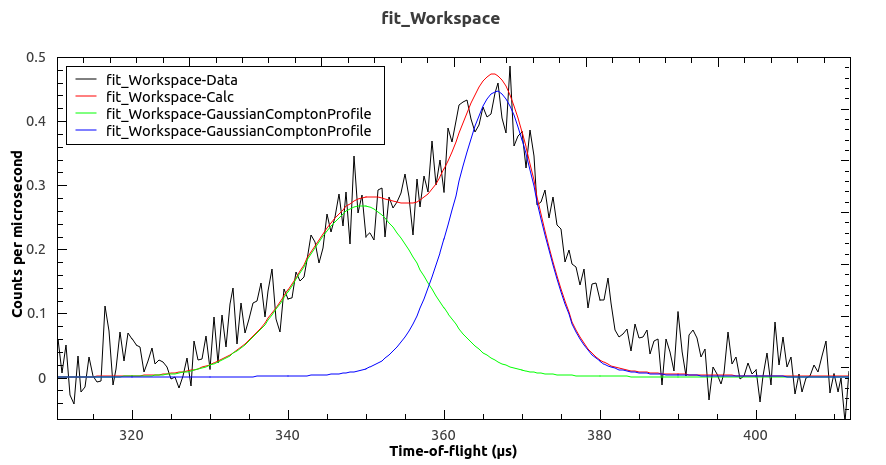
\includegraphics[width=0.6\textwidth]{img/gaussian-fit-example.png}
\caption{Plot of the fitted time-of-flight data from the sum runs 14188-14195 at the scattering angle of 163 degrees for a sample of ZrH$_2$. The black line shows the original data, the red line shows the fit to the data in red, and the individual contributing peaks are in green (aluminium) and blue (zirconium)}
\label{fig:gaussian-example-fit}
\end{figure}

\begin{listing}[H]
\begin{minted}[frame=lines,linenos=true,fontsize=\footnotesize]{python}
fit_options = ncs.FitOptions()
fit_options.workspace_index = 0
fit_options.bad_data_error = 1e6

mass1 = {'value':27.0,  'widths':[12,14.4, 16], 'function':'Gaussian', }
mass2 = {'value':91, 'widths':[24, 26.6, 28], 'function':'Gaussian'}
fit_options.masses = [mass1, mass2]

ncs.preprocess(raw_ws, fit_options)
reduced_chi_square, params_ws = ncs.run_fit(raw_ws, fit_options)
ncs.display_fit_output(reduced_chi_square, params_ws,fit_options)
\end{minted}
\caption{Example script for setting up a fit to the ZrH$_2$ sample using ncs.py. The mass of aluminium and zirconium are fitted using the Gaussian fit function. In this example, the widths of each of the masses has been fixed to a range of values using the ``widths'' attribute}
\label{lst:fit-setup}
\end{listing}

The momentum distribution of atoms has a strictly Gaussian shape only when bound by isotropic harmonic forces. The shape of the momentum distribution $n(p)$ \cite{mayers2004vesuvio}, is of interest as this contains information about the anisotropy of the binding and anharmonic effects \cite{andreani2005measurement}. In this case the data can be fitted using the \textit{GramCharlier} function. 

Setting up such a fit is very similar to the procedure described for the Gaussian approximation. Each mass being fitted using the expansion requires some additional parameters describing the hermite coefficients to be used in the fit and what the Final State Effects (FSE) coefficient should be tied too. See appendix \ref{sec:fit-options} for more details on the available options. Listing \ref{lst:fit-gram-charlier-setup} shows an example of setting up such a fit using the data for the ZrH$_2$ sample.

\begin{listing}[H]
\begin{minted}[frame=lines,linenos=true,fontsize=\footnotesize]{python}
fit_options = ncs.FitOptions()
fit_options.workspace_index = 0
fit_options.bad_data_error = 1e6

mass1 = {'value':1.0079, 'widths':[2,5,7], 'function':'GramCharlier', 
         'hermite_coeffs':[1,0,0],'k_free':False, 'sears_flag':1}
mass2 = {'value':27.0,  'widths':14.4, 'function':'Gaussian', }
mass3 = {'value':91, 'widths':26.6, 'function':'Gaussian'}
fit_options.masses = [mass1, mass2, mass3]

ncs.preprocess(raw_ws, fit_options)
reduced_chi_square, params_ws = ncs.run_fit(raw_ws, fit_options)
ncs.display_fit_output(reduced_chi_square, params_ws,fit_options)
\end{minted}
\caption{Example script for setting up a fit to the ZrH$_2$ sample using ncs.py. In this example, the widths of each of the masses except hydrogen has been fixed using ``widths'' attribute}
\label{lst:fit-gram-charlier-setup}
\end{listing}


\subsection{Fitting to determine momentum distributions}
\label{subsec:fitting-momentum-distributions}
In order to fit the data to determine the momentum distribution the raw data needs to first be normalised by the area of the peak. This removes the effects of different detector efficiencies and solid angles. The Mantid algorithm \textit{NormaliseByPeakArea} has been created to handle this step. This algorithm effectively directly replaces the implementation of the \textit{isofile} command in the original data analysis package \cite{mayers2010user}. This algorithm will:

\begin{enumerate}
\item Transform the fitted data to y-space using the algorithm \textit{ConvertToYSpace} for a single mass.
\item Fit the peak in y-space.
\item Divide the time-of-flight data by the area of the fitted peak in momentum space.
\end{enumerate}

\begin{figure}[H]
\centering
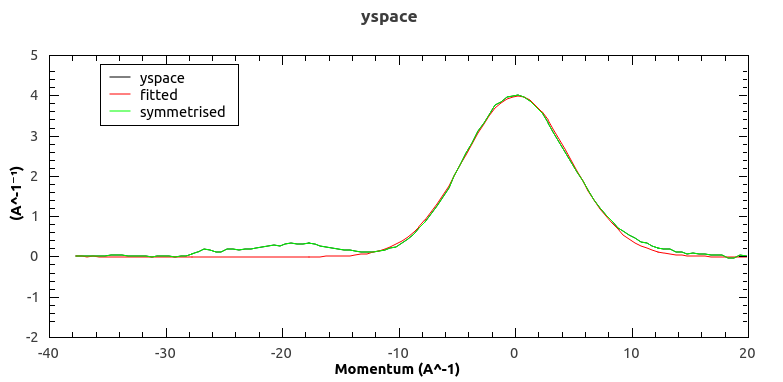
\includegraphics[width=0.6\textwidth]{img/yspace-norm.png}
\caption{Plot of the time-of-flight data normalised and converted to y-space as the black line (behind the green). The red line shows the fit to the peak and the green line shows the symmetrised workspace which is in good agreement with y-space data.}
\label{fig:yspace-norm}
\end{figure}

The \textit{NormaliseByPeakArea} algorithm produces four workspaces:

\begin{itemize}
\item \textbf{OutputWorkspace - } This workspace is the time-of-flight workspace supplied as input to the algorithm normalised by the area of the fitted peak.
\item \textbf{YSpaceDataWorkspace - } This is the time-of-flight workspace converted to y-space using the \textit{ConvertToYSpace} algorithm.
\item \textbf{FittedWorkspace - } The values of the fit to the data.
\item \textbf{SymmetrisedWorkspace - } The time-of-flight workspace converted to y-space and symmetrised about zero. As the momentum distribution should be symmetric about the origin this workspace should match the \textit{YSpaceDataWorkspace}.
\end{itemize}

\begin{listing}[H]
\begin{minted}[frame=lines,linenos=true,fontsize=\footnotesize]{python}
normalised, yspace, fitted, symmetrised = \
	NormaliseByPeakArea(InputWorkspace=raw_ws, Mass=1.0079,Sum=True)
\end{minted}
\caption{Example python code showing how to run the \textit{NormaliseByPeakArea} algorithm.}
\label{lst:normalise-peak-area}
\end{listing}

The final step in analysis is to simultaneously fit data across all detectors using the normalised workspace created as part of the previous section while keeping the widths of each peak tied. This roughly emulates the corresponding section described in Ref. \cite{mayers2010user} as the \textit{isofileu} program. This global fitting option is still currently under development.


\section{Diffraction}
\label{sec:diffraction}
Diffraction on VESUVIO is not yet fully implemented within Mantid. As the reduction of diffraction data is fairly trivial in comparison to the other requirements of VESUVIO data analysis, this can be handled by the existing IndirectDiffractionReduction routine that is used by other indirect geometry instruments. Preliminary trials with the existing implementation for other indirect instruments have shown that this should simply be a matter of adding the appropriate parameters for monitor thickness, attenuation, and area to VESUVIO's instrument parameter file.

\section{Resolution Calculation}
Calculation of the resolution of a particular mass in a sample can be performed using the \textit{calculate\_resolution} function in ncs.py. This uses the same method to calculate the resolution that is used in the fit function described in section \ref{sec:fitting}. The output of running this function is a workspace with a single spectrum for the calculated resolution. Figure \ref{fig:resolution} shows a plot of the resolution for hydrogen and listing \ref{lst:resolution} shows the python code that generated the workspace shown in the plot.

\begin{figure}[H]
\centering
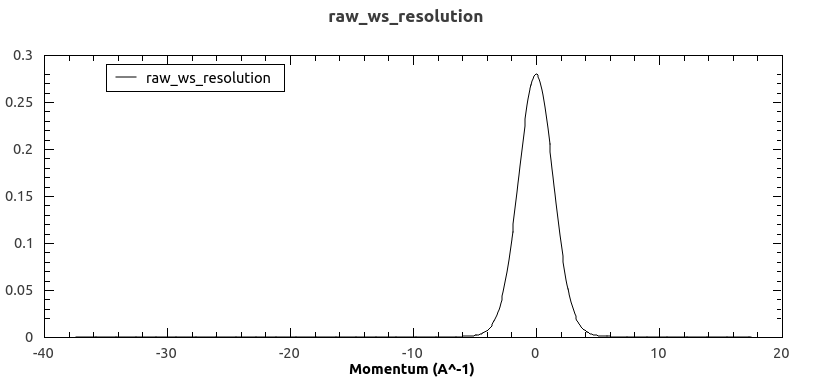
\includegraphics[width=0.6\textwidth]{img/resolution.png}
\caption{Plot of the resolution workspace generated from listing \ref{lst:resolution}.}
\label{fig:resolution}
\end{figure}


\begin{listing}[H]
\begin{minted}[frame=lines,linenos=true,fontsize=\footnotesize]{python}
import ncs

runs = "14188-14195"
spectra = "135-198"
diff_type="SingleDifference" # Allowed values=Single,Double,Thick
ip_file = "IP0004_10.par"

raw_ws = LoadVesuvio(Filename=runs, SpectrumList=spectra,
		     Mode=diff_type,InstrumentParFile=ip_file)
raw_ws = CropWorkspace(raw_ws,XMin=50.0,XMax=562.0)

mass = 1.0079
raw_ws = ConvertToYSpace(raw_ws, mass)
ncs.calculate_resolution(raw_ws, mass)
\end{minted}
\caption{Example script showing how to calculate the resolution for a particular mass.}
\label{lst:resolution}
\end{listing}

\section{Calibration of Instrument Parameters}
\label{sec:calibration}
The calibration routines for VESUVIO have been implemented as two Mantid algorithms following the procedures described in Ref. \cite{mayers2011calibration}. The first algorithm, called \textit{EVSCalibrationFit}, is used to fit sample data in order to accurately obtain the values of the parameters for the instrument. A second Mantid algorithm built on top of the first is used to set up and run the fitting does the actual calculation of the instrument parameters called \textit{EVSCalibrationAnalysis}. These two algorithms should only be run by instrument scientists and a calibration parameter file does not need to be recreated for every data analysis session.


\begin{figure}[H]
\centering
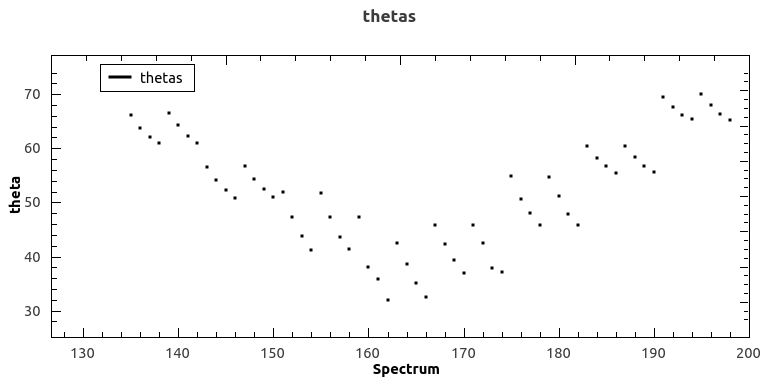
\includegraphics[width=0.6\textwidth]{img/calib-theta.png}
\caption{Plot showing the calculated scattering angle from a Pb sample.}
\label{fig:calib-theta}
\end{figure}

The calibration fit program can either fit using a list of incident energies to calculate the expected centre point of a recoil peak in time-of-flight data or by taking a list of $d$-spacings and calculating the position of Bragg peaks. The algorithm also requires a file containing a set of reference parameters with which to calculate the expected peak positions. This is analogous to the procedures described in Ref. \cite{mayers2011calibration} where hand measured parameters were used as starting values and the fitting program used these to incrementally converge on the true value of the instrument parameters.

The analysis program makes use of the fit program to fit all of the parameters in the order defined by the original VESUVIO calibration paper \cite{mayers2011calibration}, starting with the incident flight path and time delay using well defined uranium sample runs, then computing the values of the final energy and hence the final flight path and finally the scattering angles for all detectors.

\section{GUI}
\label{sec:GUI}
VESUVIO does not currently have any GUI support within Mantid. Focus on development has been to get the underlying reduction and analysis routines working before focusing on usability. The current plan is for VESUVIO to have a completely new GUI listed under the indirect geometry section of Mantid. The current design would be to have a series of three tabs on the interface which would each deal with a separate part of reduction and analysis.

\begin{itemize}
\item \textbf{Loading:} This tab would broadly handle the procedures described in section \ref{sec:viewtof} and would provide a user interface for using the LoadVesuvio algorithm to get raw data into Mantid as well as providing plotting functions for examining the captured time-of-flight data.

\item \textbf{Corrections:} The corrections tab would provide a user interface for calculating both multiple scattering and gamma background corrections and applying them to data loaded in the first tab.

\item \textbf{Fitting:} The fitting interface is the most complex in the series. This will provide support for setting up a fit using the same procedures used in the ncs.py module, but in a more user friendly manner than the current implementation achieves. This would provide support for both the Gaussian and Gram-Charlier functions as well as the ability to set the intensity constraints and Hermite polynomial expansion coefficients.
\end{itemize}

This is simply a loose plan based on previous discussions. The number and function of the tabs on the interface may change as development progresses. A proper design cannot be produced until the underlying framework is finalised. For example, there is a currently goal to support fitting a sample directly in y-space. It may be possible to integrate this with the fitting tab mentioned above, or depending on requirements, may be split to a fourth tab. Global fitting may well also require yet another separate interface.

\section{Visualisation}
\label{sec:visualisation}
VESUVIO analysis requires a few custom plotting commands to display data in ways which are not currently supported by the general Mantid framework. To solve thos, user can examine their data more easily with some helper functions which exist in the ncs\_plotting.py module. This is provides a single plot function with options to plot data by spectra, scattering angles, or detector banks. In future releases it is hoped that these can become properly integrated into the general Mantid framework.

\begin{figure}[H]
\centering
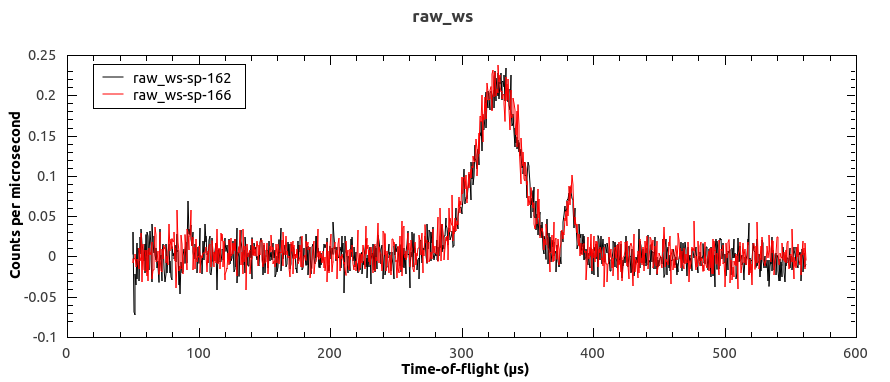
\includegraphics[width=0.6\textwidth]{img/plot-angle.png}
\caption{Plot of some raw time-of-flight data using the ncs\_plotting module using the script in listing \ref{lst:plot-angle}. Checking the spectrum numbers in the key shows that the scattering angles of 33$^\circ$ and 32$^\circ$ have been plotted.}
\label{fig:plot-angle}
\end{figure}

Appendix \ref{sec:plotting-options} lists all of the currently supported plotting commands. This replicates the functionality for the various plotting routines that the old data analysis package had. The listing \ref{lst:plot-angle} shows a basic example of plotting some spectra from a raw workspace by angle using the ncs\_plotting module. Figure \ref{fig:plot-angle} shows the resulting plot.

\begin{listing}[H]
\begin{minted}[frame=lines,linenos=true,fontsize=\footnotesize]{python}
import ncs_plotting

runs = "14188-14195"
spectra = "3-195"
diff_type="SingleDifference" # Allowed values=Single,Double,Thick
ip_file = "IP0004_10.par"

raw_ws = LoadVesuvio(Filename=runs, SpectrumList=spectra,
		     Mode=diff_type,InstrumentParFile=ip_file)
raw_ws = CropWorkspace(raw_ws,XMin=50.0,XMax=562.0)

ncs_plotting.plot(raw_ws, angles=(30,35))
\end{minted}
\caption{Example python code showing how to plot spectra in a workspace within the scattering range of 30-35$^\circ$ using the ncs\_plotting module.}
\label{lst:plot-angle}
\end{listing}

\clearpage
\section*{Acknowledgments}
The author would like to thank M. Gigg, A. Seel, for their knowledgeable assistance in producing this report and for aiding with the parts of the implementation the author had a hand in, and M. Gigg and R. Tolchenov who wrote the majority of the implementation presented in this document. Many thanks to M. Krzystyniak for his contributions and  corrections, particularly in regard to VESUVIO theory. I would also like to thank S. Mukhopadhyay for her contributions to the report.

\clearpage
\bibliographystyle{unsrtnat_corrected}
\bibliography{references}

\clearpage
\begin{appendices}
\section{Fit Options}
\label{sec:fit-options}
The following two tables list all of the current options that may be supplied to the \textit{FitOptions} object created using ncs.py. The first table shows the general parameters for the fit, while the second table lists the options used to define a single mass used as part of a fit.

\begin{table}[H]
\centering
\begin{tabular}{ l p{12cm}}
Name & Description \\ \hline
\textit{smooth\_points} & Number of data points to use in the SmoothData algorithm in the pre-processing function. If not set the data will not be smoothed. \\ \hline
\textit{bad\_data\_error} & If set, the data will be masked if it falls outside of this error tolerance.\\ \hline
\textit{background\_function} & The type of background to use in fitting. By default this is set to use the Polynomial background function. \\ \hline
\textit{background\_order} & The order of the background to use.\\ \hline
\textit{masses} & A dictionary of parameters for each mass supplied to the fit. This should include the atomic weight, function to fit (either \textit{Gaussian} or \textit{GramCharlier}) any any other parameters required by the function. \\ \hline
\textit{constraints} & Constraints on the intensity of each mass peak. \\ \hline
\textit{workspace\_index} & The index in the workspace to fit to. \\ \hline
\textit{output\_prefix} & String which is prefixed to output workspaces created from the fitting. \\ \hline
\textit{global\_fit} & Whether or not to perform a multi-dataset (global) fitting of the data. \\ \hline
\end{tabular}
\caption{Table listing the different fitting options available in the FitOptions class}
\label{table:fit-parameters}
\end{table}

\begin{table}[H]
\centering
\begin{tabular}{ l p{12cm}}
Name & Description \\ \hline
\textit{value} & The atomic weight of the mass in amu \\ \hline
\textit{widths} & The width of the peak. If this is set to a single number the width will be fixed to that value. If it is set to an iterable (tuple or list) of three values the middle value is the starting value and the first and last values are the constraints on the parameters' fit. \\ \hline
\textit{function} & The function to use to fit this mass. Options are currently either \textit{Gaussian} or \textit{GramCharlier}. \\ \hline
\textit{hermite\_coeffs} & Only applicable when using \textit{GramCharlier}. This is a list of coefficients for each mass being fitted. If set to one the term is included within the fit. If set to zero it is excluded from the fit\\ \hline
\textit{k\_free} & Only applicable when using \textit{GramCharlier}. If this flag is set to true the FSE (``Final State Effects'') coefficient is not tied to a value. If false it is set to a value dependant on the \textit{sears\_flag}.\\ \hline
\textit{sears\_flag} & Only applicable when using \textit{GramCharlier}. If the \textit{k\_free} flag is set to false, this flag will control what the FSE coefficient gets tied too. If set to one it is tied to $width\times\sqrt{\frac{2}{12}}$ which is harmonic limit of the magnitude of the FSEs\\ \hline
\end{tabular}
\caption{Table listing the options for defining a mass to be fitted.}
\label{table:mass-parameters}
\end{table}

\clearpage
\section{Plotting Options}
\label{sec:plotting-options}

The following table summarises the plotting options available in the \textit{plot} routine in the ncs\_plotting.py module.
\begin{table}[H]
\centering
\begin{tabular}{ l p{15cm}}
Name & Description \\ \hline
\textit{spectra} & Plot a single spectrum or, given a list of indices, plot any number of spectra. \\ \hline
\textit{angles} & Plot by scattering angle given a list/tuple of size two specifying the minimum and maximum angles in the range. \\ \hline
\textit{bank} & Plot a single bank or, given a list of bank numbers, plot any number of banks with the inclusive range of 1-8. \\ \hline
\textit{errors} & Create the plot with error bars shown. Default is false. \\ \hline
\textit{sum} & Sum all spectra falling within the range defined by the angle/spectra/bank options. This is applied independently to each workspace is there is more than one. Default is false.\\ \hline
\textit{fig} & If supplied the a new window will not be created, but the new plot will be attached to the existing figure referenced by \textit{fig}\\ \hline
\textit{clrfig} & If supplied the given window will be clear before the new plot is drawn. \\ \hline
\end{tabular}
\caption{Table listing the options that can be used in conjunction with the plot function.}
\label{table:plotting-parameters}
\end{table}

\end{appendices}
\end{document}